%-------------------------------------------------------------------------
% Design Project Input/Output Module Description
%-------------------------------------------------------------------------

\clearpage
\section{Heart Rate Input Module}
\label{sec-input-heart}

This input module enables your IoT device to sense your heart beating.
Heart rate monitors are useful for monitoring heart rate in a variety of
applications, including exercise and fitness (targetting a healthy heart
rate), injury rehabilitation, hospital monitoring systems, and
biotelemetry. The Polar T34 Non-Coded Heart Rate Transmitter (the
wearable chest strap) monitors and then wirelessly transmits your heart
rate data from the chest strap to the Polar Heart Rate Receiver (the
small green IC), which can then communicate data to the Arduino. The
heart rate monitor works by detecting electrical heart muscle signals as
the heart beats. The chest strap can sense these electric signals when
the two contacts are moistened and are in direct contact with your skin,
and it sends a pulsed wireless signal to the receiver when it detects a
beat.

A sample circuit and Arduino code is shown below to get you started.
There is no need for any extra components. The example code will print
"Heartbeat" on the serial monitor whenever a heart beat is detected.
After setting up the circuit and programming the Arduino, you can secure
the chest strap to your partner's chest, just below the chest muscles,
and buckle the strap together. Moisten the two grooved electrode areas
on the back of the chest strap. Check that the wet grooved areas are
firmly against the skin and that the word "Polar" is right-side up. The
moistened grooved areas activate the transmitter, so make sure to dry
the sensor when not in use. After securing the chest strap, open the
serial monitor, use your hand to find your own pulse, and verify that
"Heartbeat" is printed at the same time your heart is beating.

\vspace{0.1in}
\begin{minipage}[t]{0.49\tw}
  \vspace{0pt}
  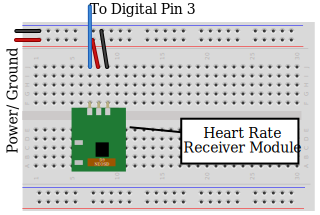
\includegraphics[width=\tw]{input-heart-annotated.svg.pdf}

  \vspace{0pt}
  
\includegraphics[width=\tw]{heart.jpg}
\end{minipage}
\hfill
\begin{minipage}[t]{0.49\tw}
  \vspace{0.1in}
  \begin{Verbatim}[gobble=3,fontsize=\small]
    int pin_heart = 3;
    byte old_sample, sample;

    void setup() {
      Serial.begin(9600);
      pinMode (pin_heart, INPUT);

      Serial.println("Waiting for heart beat...");

      // Wait until a heart beat is detected
      while ( !digitalRead(pin_heart) ) {};
      Serial.println ("Heart beat detected!");
    }

    int heartbeat_count;

    void loop() {
      sample = digitalRead(pin_heart);
      if (sample && (old_sample != sample)) {
        Serial.print("Heartbeat: ");
        Serial.println( heartbeat_count );
        heartbeat_count++;
      }
      old_sample = sample;
    }

  \end{Verbatim}
\end{minipage}

